\documentclass[letterpaper,10pt]{article}

\usepackage{titling}
\usepackage{listings}
\usepackage{url}
\usepackage{setspace}
\usepackage{subfig}
\usepackage{sectsty}
\usepackage{pdfpages}
\usepackage{colortbl}
\usepackage{multirow}
\usepackage{multicol}
\usepackage{relsize}
\usepackage{amsmath}
\usepackage{wasysym}
\usepackage{fancyvrb}
\usepackage{amssymb}
\usepackage{ifsym}
\usepackage{amsmath,amssymb,amsthm,graphicx,xspace}
\usepackage[titlenotnumbered,noend,noline]{algorithm2e}
\usepackage[compact]{titlesec}
\usepackage{XCharter}
\usepackage[T1]{fontenc}
\usepackage{tikz}
\usetikzlibrary{arrows,automata,shapes,trees,matrix,chains,scopes,positioning,calc}
\tikzstyle{block} = [rectangle, draw, fill=blue!20, 
    text width=2.5em, text centered, rounded corners, minimum height=2em]
\tikzstyle{bw} = [rectangle, draw, fill=blue!20, 
    text width=4em, text centered, rounded corners, minimum height=2em]

\definecolor{namerow}{cmyk}{.40,.40,.40,.40}
\definecolor{namecol}{cmyk}{.40,.40,.40,.40}

\let\LaTeXtitle\title
\renewcommand{\title}[1]{\LaTeXtitle{\textsf{#1}}}


\newcommand{\handout}[5]{
  \noindent
  \begin{center}
  \framebox{
    \vbox{
      \hbox to 5.78in { {\bf ECE356: Database Systems } \hfill #2 }
      \vspace{4mm}
      \hbox to 5.78in { {\Large \hfill #4  \hfill} }
      \vspace{2mm}
      \hbox to 5.78in { {\em #3 \hfill} }
    }
  }
  \end{center}
  \vspace*{4mm}
}

\newcommand{\lecture}[3]{\handout{#1}{#2}{#3}{Lecture #1}}
\newcommand{\tuple}[1]{\ensuremath{\left\langle #1 \right\rangle}\xspace}

\addtolength{\oddsidemargin}{-1.000in}
\addtolength{\evensidemargin}{-0.500in}
\addtolength{\textwidth}{2.0in}
\addtolength{\topmargin}{-1.000in}
\addtolength{\textheight}{1.75in}
\addtolength{\parskip}{\baselineskip}
\setlength{\parindent}{0in}
\renewcommand{\baselinestretch}{1.5}
\newcommand{\term}{Winter 2018}

\singlespace


\begin{document}

\lecture{ 20 --- Query Optimization and Plan Selection }{\term}{Jeff Zarnett}

\section*{Query Optimization}

The final advanced subject in query optimization is complex enough that it deserves a more detailed look: join elimination. So much of the previous examination has focused on the cost of the join and that has highlighted in a real way just how expensive it is to perform a join. For this reason, good optimizer routines will attempt to eliminate the join altogether if it can be skipped. The optimizer can only do this if there is certainty that the outcome will not be affected by not doing the join. We will shortly see how that is accomplished.

\subsection*{Join Elimination}

You may ask, of course, why should the optimizer do this work at all? Why not simply count on the developers who wrote the SQL in the first place to refactor/change it so that it is no longer so inefficient? That would be nice but would you also like a pony?  Developers make mistakes, as you know, or perhaps some legacy code cannot be changed for some reason. Regardless, SQL is a language in which you specify the result that you want, not specifically how to get it. If there is a more efficient route, then it's worth taking from the point of view of the database server. The same logic applies in the compiler, incidentally; if you ask for some operation that the compiler knows it can replace with an equivalent but faster operation, why wouldn't you want that? Compilers don't admonish the user for writing code that it has to transform into a faster equivalent, they just do that transparently\footnote{Of course, if you'd like a peek behind the curtain to see what compiler optimizations do, ECE~459, Programming for Performance, does examine some parts of this!}.

Our guide in this is~\cite{joinelim}. We will examine some real SQL queries to see how we can get rid of a total unnecessary join. This join can only be removed if the database server can prove that the join is not needed and that therefore the removal of this operation has no impact on the outcome.


Consider a statement that looks like this: \texttt{SELECT c.* FROM customer AS c JOIN address AS a ON c.address\_id = a.address\_id;} This gets customer information and joins with those where there are addresses on file. This is an inner join and as presented simply we cannot do anything with this information. We need to make sure that the customer data has a matching row.

If, however, a new piece of information is considered, it changes everything entirely. Suppose that we have a foreign key defined from customer's \texttt{address\_id} to the address \texttt{id} field. If nulls are not permitted then we know for sure that every customer has exactly one record in the address table and therefore the join condition is not useful and may be eliminated. This means we could in fact replace that query with \texttt{select * from customer;} with no need for any references to the join table at all. That would be much, much faster since it is a simple select with no conditions.

The foreign key and not null constraints on the address ID field of the customer make it possible for the optimization of the join elimination to occur.

An outer join constraint can be removed as well. Imagine the query said this: \texttt{SELECT c.* FROM customer AS c LEFT OUTER JOIN address AS a ON c.address\_id = a.address\_id;}. All tuples are fetched from customer whether or not there is an associated address. Once again, if the foreign key constraint and not-null properties hold for this field it means that we can perform the equivalent transformation and replace the join query with a simple unqualified select. 

Suppose the foreign key constraint is removed. Does that change anything? No -- a unique constraint on the address would be sufficient for us to conclude that the join means no duplication of rows in customer will take place. Therefore it can once again be replaced with the simple \texttt{select * from customer;}.

If, however, both constraints are removed and we cannot be sure that there is at most one address corresponding to a customer, then we have no choice but to do the join.

For an even wilder example, when an outer join occurs with distinct keyword: in a many-to-many relationship (the example in the source material is about actors and films) then outer join would produce duplicate tuples. The query asks for a listing of actor names. It is an outer join query (which I confess makes very little sense: why do you care about the films entered who have no actors in them, and why would there be any anyway?). Because it's an outer join you will even return the actors who appear in no films (also known as ``waitstaff in LA restaurants''\footnote{I apologize if that was overly mean.}). And thus potentially a lot of duplicates that are eliminated. 

This last example is a bit forced, at least in my opinion. Why would you query all actors whether or not they had been in a film by referencing films? If you don't care whether they had been in a film, why do you even look at the films table... Anyway, this sort of thing could happen in an application where the SQL statement is composed by some if-statement logic where there are multiple checkboxes like ``appears in a film'' and ``does not appear in film'' and two conditions are added (like ``incoming = true OR incoming = false'').

Obviously, the more complex the query, the harder it is to determine whether or not a particular join may be eliminated. More than that, the same queries written exactly the same on a database in which the constraints have not been added would not be eligible for the join elimination optimization. In the inner join example, the foreign key and not null constraints, for example, are beneficial. This reveals a second purpose why constraints are valuable in the database. In addition to allowing us to enforce logical rules of the application inside of the database, it allows queries to be completed more efficiently.

Perhaps an analogy helps. You are asked to search through the library to find all copies of the book ``Harry Potter and the pthread House Elves''. That is a plausible task. But, suppose that you know as well there is a rule that this library will keep only one copy of that book ever. If that is the case, as soon as you have found the single copy of that book, you can stop looking (no need to check more ``just in case''). This sort of optimization is very similar in that the rules let us avoid doing unnecessary work and that is a big part of the optimization routine.

The following short table tells us a bit about what database servers implement join elimination (hint: Not MySQL). The original is from ~\cite{joinelim} but I've modified it a bit to make it more colourblindness-friendly (mostly by making it grey instead of red and green):

\begin{center}
	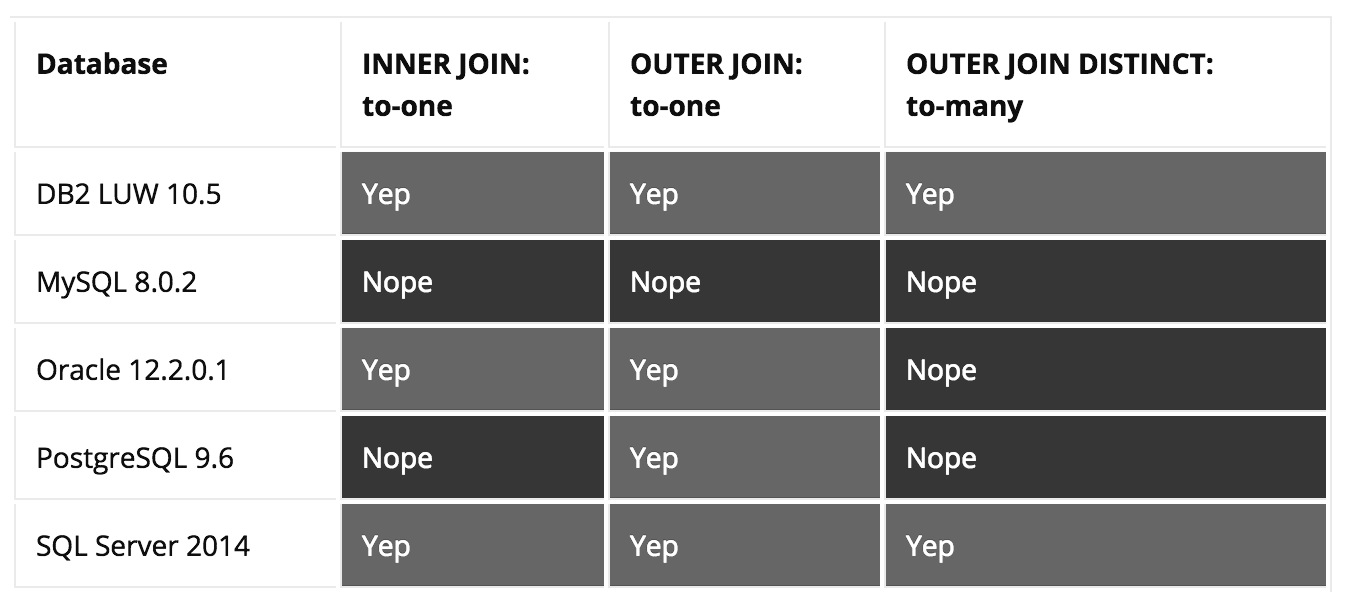
\includegraphics[width=0.7\textwidth]{images/joinelim-support}
\end{center}

For those databases that do not support automatic join elimination developers simply have to ``do better''. 

\section*{Evaluation Plan Selection}

It was perhaps oversimplifying to have said earlier that choosing a plan was just as simple as picking the one with the lowest cost. There is a little bit more to it than that. There is always a catch. There about choosing the one with the lowest cost is correct (generally) but the difficulty is in devising and calculating all possible evaluation plans. These operations are not free in terms of CPU usage or time and it is possible to waste more time on analysis than choosing a better algorithm would save. 

A simplified approach, then, focuses just on what order in which join operations are done and then how those joins are carried out. The theory is that the join operations are likely to be the slowest and take the longest, so any optimization here is going to have the most potential benefit.

We already know that the order of joins in a statement like $r_{1} \bowtie r_{2} \bowtie r_{3}$ is something the optimizer can choose. In this case there are 3 relations and there are 12 different join orderings. In fact, for $n$ relations there are $\dfrac{2(n-1)!}{(n-1)!}$ possible orderings~\cite{dsc}. Some of them, are obviously symmetric which reduces the number that we have to calculate, since $r_{1} \bowtie r_{2}$ is not different from $r_{2} \bowtie r_{1}$ (in relational algebra). In any case, even if we can cut down the symmetrical cases the problem grows out of hand very quickly when $n$ gets larger. 

Once more than three relations are affected by a join query it may be an opportunity to stop and think very hard about what is going on here, because this is quite unusual if the database design is good. The database server may want to ask why do you have a join query that goes across six or eight or twelve relations, but the database server (sadly) does not get to write the developers a nasty resignation letter saying that it can't continue to work this hard due to the negative effects on its health. It will dutifully do the work you asked it to and even try to make the best of this inefficient situation by optimizing it. But clearly it cannot examine all (non-symmetric) approaches and choose the optimal one. It would take too long.

Fortunately, we can create an algorithm that can ``remember'' subsets of the choices. If we have, for example, $r_{1} \bowtie r_{2} \bowtie r_{3} \bowtie r_{4} \bowtie r_{5}$ and the database server does not segmentation fault in disgust, we can break that down a bit. We could compute the best order for a subpart, say $(r_{1} \bowtie r_{2} \bowtie r_{3})$ and then re-use that repeatedly for any further joins with $r_{4}$ and $r_{5}$~\cite{dsc}. This ``saved'' result can be re-used repeatedly turning our problem from five relations into two three-relation problems.

This is a really big improvement, actually, considering how quickly the factorial term scales up. The trade-off for this approach is that the resultant approach may not be globally optimal (but instead just locally optimal). If $r_{1} \bowtie r_{4}$ produces very few tuples, it may be maximally efficient to do that join computation first, a strategy that will never be tried in an algorithm where $r_{1}$, $r_{2}$, and $r_{3}$ are combined to a subexpression for evaluation. 

Remember though, this is as estimating process. The previous statement that said $r_{1} \bowtie r_{4}$ produces very few tuples as if it is a fact. The optimizer does not know that for sure and must rely on estimates where available. So even though the optimizer may, if it had tried all possibilities, determined that $r_{1} \bowtie r_{4}$ produces the fewest tuples and should be joined first, it is possible that estimate was off and the actual cost of a different plan was lower.

A simple pseudocode algorithm for using dynamic programming to optimize join orders is below from~\cite{dsc}. In this, imagine that there exists a structure \texttt{result} that contains both a plan and a cost element. This result is stored in some array or other data structure for future retrieval. This recursive algorithm has $O(3^{n})$ behaviour which is... well... it's not going to win algorithm of the year.

\begin{verbatim}
procedure find_plan( subquery S ) 
  if current subquery S result has already been computed
    return previously computed result for S
  end if

  declare variable result

  if current subquery S contains no joins
    set result.plan for S to best way of accessing this relation
    set result.cost for S this relation based on plan
  else 
    for each non empty subset S1 of current relation S that is not equal to S
      variable r1 = find_plan( S1 ) 
      variable r2 = find_plan( S - S1 )
      A = best algorithm for joining r1 and r2
      cost = r1.cost + r2.cost + cost of A
      if cost less than current best plan for S
        result.plan = execute r1, execute r2, join using A
        result.cost = cost
      end if  
    end for
   end if
return result
\end{verbatim}

This is perhaps a bit hard to read and may require some explanation. The procedure checks if there has already been a result computed for this and if it is then there is no sense in re-doing that work. Use the already known result instead. Otherwise we will break the query down into smaller and smaller parts until we get down to just one relation: retrieving the matching part of that relation is computed. Then we can go up a level and find the best way to join that with the result (which itself may need to be broken down). This recursive procedure will eventually produce a result for how long it will take to perform the series of joins.

The sort order in which tuples are generated is important if the result will be used in another join. A sort order is called \textit{interesting} if it is useful in a later operation. If $r_{1}$ and $r_{2}$ are being computed for a join with $r_{3}$ it is advantageous if the combined result $r_{1} \bowtie r_{2}$ is sorted on attributes that match to $r_{3}$ to make that join more efficient; if it is sorted by some attribute not in $r_{3}$ that means an additional sort will be necessary~\cite{dsc}.

With this in mind it means that the best plan for computing a particular subset of the join query is not necessarily the best plan overall, because that extra sort may cost more than was saved by doing the join itself faster. This increases the complexity, obviously, of deciding what is optimal. Fortunately there are, usually anyway, not too many interesting sort orders~\cite{dsc}. 

\subsection*{Generating Alternatives}

Join order optimization is a big piece of the puzzle but it's not the only thing we can do in query evaluation. Let's briefly revisit the subject of how equivalent queries are formed. We already decided it is too expensive to try out all equivalent queries, but perhaps we are determined to try to at least generate lots of alternatives. The textbook~\cite{dsc} summarizes some strategies from the Volcano research project that would make it possible to generate a larger number of plans than we might otherwise be able to. We need four things.

\begin{enumerate}
	\item A way of storing expressions that reduces duplication and therefore keeps down the amount of space needed to store the various queries.
	\item A way of detecting duplicate derivations of the same expression.
	\item A way of storing optimal subexpression evaluation plans so that we don't have to recompute them.
	\item An algorithm that will terminate early the evaluation of a particular plan if it is already worse than the cheapest plan so far found. 
\end{enumerate}

The details are obviously a bit complex. Most of this is beyond what we will discuss in this course, but some of those things we have already seen. For example, the algorithm earlier has got a way of storing evaluations of sub expressions so that we can re-use them. It could be modified to terminate earlier if, for example, the individual costs of \texttt{r1} or \texttt{r2} were already larger than the known stored plan.

\subsection*{Nested Subqueries}

On the subject of generating alternatives, if possible, nested subqueries will be transformed into an alternative representation: a join query. To summarize the rather long story, if evaluated the ``slow'' way the subquery needs to be run a lot of times. Thus, to make it faster, we would prefer to turn it into a join (which we already know how to handle). If really necessary we can run the subquery once and use that temporary relation in a join (where exists or ``in'' predicates may fall into this category).

Suffice it to say that transformation of nested queries is complicated and it may mean that the optimizer is unable to find some efficient route for executing the desired query if the query is complex. If possible, nested queries should be avoided. Sometimes you don't have much choice however. Amusingly, many years ago, MySQL did not support subqueries and that was one way to force people to come to grips with how to use joins. But somehow I do not think MySQL was intentionally doing anyone a favour, any more than having a terrible optimizer ``forces'' developers to write better queries. 


\subsection*{Shortcuts}

Now we will talk about some heuristic rules (guidelines, really) that we have definitely mentioned earlier when we talked about, for example, how to perform a selection. Now we can actually discuss them more formally.

\paragraph{Perform selection early.} No surprises here: the sooner we do a selection, the fewer tuples are going to result and the fewer tuples are input to any subsequent operations. Performing the selection is almost always an improvement. Chances are we get a lot of benefit out of selection: it can cut a relation down from a very large number of tuples to relatively few (or even one). 

There are exceptions, however. One from~\cite{dsc}: suppose the query is $\sigma_{\theta}( r \bowtie s )$ where $\theta$ refers only to attributes in $s$. If we do the selection first and (1) $r$ is small compared to $s$ and (2) there is an index on the join attributes of $s$ but not on those used by $\theta$ then the selection is not so nice. It would throw away some useful information and force a scan on $s$; it may be better to do the join using the index and then remove tuples with the selection.

\paragraph{Perform projection early.} Analogous to the idea of doing selection early, performing projection early is good because it tosses away information we do not need and means less input to the next operations. Just like selection, however, it is possible the projection throws away an attribute that will be useful. If the query does not ask for the join attribute in the output (e.g., does it matter what a person's address ID is?) then that join attribute will need to be removed from the output but if removed too soon it makes it impossible to do the join.

\paragraph{Left-deep join orders.} Some query optimizers do not bother doing all the fanciful join optimization routines to solve which joins are best; instead they will consider join orders where each of the right operands of the join is always one of the initial relations $r_{k}$ from the provided query $r_{1} \bowtie r_{2} \bowtie ... \bowtie r_{n}$. The reasoning behind this is it takes ``only'' $O(n!)$ time to consider all left-deep orders rather than all possible join orders~\cite{dsc}. 

This is perhaps best illustrated with the following graphic, also from~\cite{dsc}:

\begin{center}
	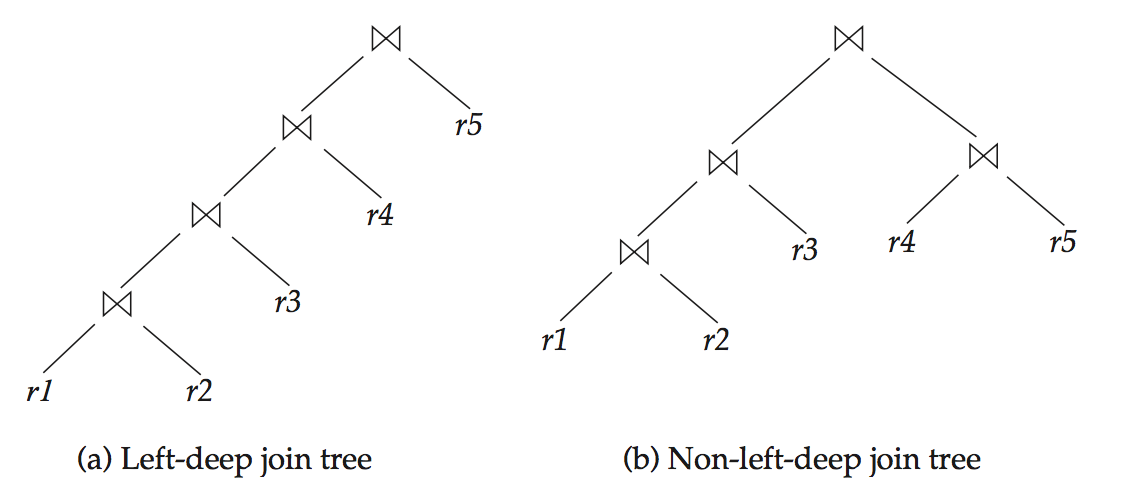
\includegraphics[width=0.6\textwidth]{images/deep-join-tree}
\end{center}

In part (a) of the diagram the joins are all shown as happening in some ascending order  from $r_{1}$ through $r_{5}$ but in reality the optimizer would consider this one possibility and then rearrange the relations through all possible arrangements to work out what is best.

\paragraph{Set limits.} Another strategy for making sure we choose something appropriate within a reasonable amount of time is to set a time limit. Optimization has a certain cost and once this cost is exceeded, the process of trying to find something better stops. But how much time to we decide to allocate? A suggested strategy from~\cite{dsc} says to use some heuristic rules to very quickly guess at how long it will be. If it will be very quick then don't bother doing any further searching, just do it. If it will be moderate in cost, then a moderate optimization budget should be allocated. If it is expensive then a larger optimization budget is warranted.

\paragraph{Plan caching.} In any busy system, common queries may be repeated over and over again with slightly different parameters. For example, \cite{dsc} suggests the following sort of query: a student wishes to query what courses they are enrolled in. If one student does this query with a particular value for student ID number, we can re-use that same evaluation plan in the future when another student does the exact same query with her student ID number instead. 

The results will be different and this query may be more expensive on the second run if, for example, the second student is taking 7 courses this term and the first student is taking 5. That is expected, all we really needed was an estimate. With that in mind, if we have actually carried out the exact query we can use the actual execution time as the updated estimate for how long it takes (or perhaps an average of the last $n$ executions of that same query if it has high variability). 


\bibliographystyle{alphaurl}
\bibliography{356}


\end{document}
